% !TEX root = ../Thesis.tex
\myChapter{Multimodal imaging for the detection of sub-micron particles in the gas-exchange region of the mammalian lung}\label{ch:XRM2008}

\newcommand{\footremember}[2]{\footnote{#2}\newcounter{#1}\setcounter{#1}{\value{footnote}}}%
\newcommand{\footrecall}[1]{\footnotemark[\value{#1}]} 

David Haberthür\footremember{ana}{Institute of Anatomy, University of Bern, Bern, Switzerland}\\
Manuela Semmler-Behnke\footremember{inhalation}{Institute for Inhalation Biology, Helmholtz Zentrum München, Germany}\\
Shinji Takenaka\footrecall{inhalation}\\
Wolfgang G. Kreyling\footrecall{inhalation}\\
Marco Stampanoni\footremember{psi}{Swiss Light Source, Paul Scherrer Institut, Switzerland}\textsuperscript{,}\footremember{eth}{Institute for Biomedical Engineering, University and ETH Zürich, Switzerland}\\
Akira Tsuda\footnote{Physiology Program, Harvard School of Public Health, US}\\
Johannes C. Schittny\footrecall{ana}\textsuperscript{,}\footnote{\href{mailto:schittny@ana.unibe.ch}{schittny@ana.unibe.ch}}\\\\
First published in: J. Phys.: Conf. Ser. 186 012040 (3pp)\\
\href{http://dx.doi.org/10.1088/1742-6596/186/1/012040}{doi:10.1088/1742-6596/186/1/012040}

\section{Abstract}
The deposition sites of inhaled aerosols in the gas-exchange region of the lung represent one of the key parameters needed for the understanding of the interaction between these particles and lung tissue. In order to develop a method for three-dimensional imaging of sub-micron particles in lung tissue we applied gold particles (200 and \SI{700}{\nano\meter}) to rat lungs by intratracheal instillation. The samples were scanned at the beamline for \acf{TOMCAT} at the \acl{SLS}. The \SI{200}{\nano\meter} particles were slightly below the detection capabilities of \acs{TOMCAT}. Therefore, their localization was obtained only by electron microscopy. At a voxel size of \SI{350}{\nano\meter} we observed single and clustered gold particles (\SI{700}{\nano\meter}) in alveoli, alveolar ducts, and small bronchioli. The locations of the gold particles were verified by transmission electron microscopical serial sections. We observed a very high correlation between these two imaging modalities. We conclude that a combination of x-ray tomographic microscopy and electron microscopy allows the full unrestricted \threed localization of particles smaller than the resolution of x-ray tomographic microscopy. We are planning to use this method for the verification of the simulation of particle deposition in the airway tree.

\section{Objective}
To study the deposition of sub-micron particles in the mammalian lung, we used \ac{SRXTM} to record tomographic images of lung samples with high resolution (\SI{350}{\nano\meter}). In addition to \ac{SRXTM}, we used conventional \ac{TEM} to obtain high resolution images (resolution smaller than \SI{1}{\nano\meter}).

\section{Materials and Methods}
We applied \SI{200}{\nano\meter} and \SI{700}{\nano\meter} gold particles to rat lungs by intratracheal instillation. Thirty minutes after instillation, the lungs were fixed with \SI{2.5}{\%} glutaraldehyde by vascular perfusion, stained according to standard protocols for \ac{TEM} and embedded in Epon. The samples were shaped to cylinders with a diameter of either 0.6 or \SI{1.2}{\milli\meter} and a length of several millimeters using a watchmakers lathe and then scanned at \ac{TOMCAT}~\cite{Stampanoni2007}, the beamline for \acl{TOMCAT} at the \acl{SLS} at the Paul Scherrer Institute in Villigen, Switzerland. The samples were scanned at a wavelength of \SI{11.5}{\kilo\electronvolt}, post processed on a 20-node Linux cluster using filtered backprojection, resulting in an image stack of 2048$\times$2048$\times$2048 pixels with isotropic voxels of \SI{350}{\nano\meter} side length. The samples were visualized in three dimensions using an isosurface computed with Imaris x64 5.72 (Bitplane AG, Switzerland) on an AMD 64-based windows computer~\cite{Tsuda2008}. After tomographic image acquisition serial sections of the sample were cut and processed for transmission electron microscopy~\cite{Mund2008}. 

\section{Results}
We have been able to observe single and clustered gold particles in alveoli, alveolar ducts, and small bronchioli while imaging them at a voxel side length of \SI{350}{\nano\meter} with the use of \ac{SRXTM} (Fig.~\ref{subfig:imaris} and \ref{subfig:slice-srxtm}). We were able to verify the locations of the observed gold particles by \ac{TEM} (Fig.~\ref{subfig:slice-em}). 

Particles with a size of \SI{200}{\nano\meter}---a size smaller than the resolution achievable at \ac{TOMCAT}---were imaged using \ac{TEM} after selecting a particular alveolus in three dimensional visualizations obtained from \ac{SRXTM} data. Thirty minutes after instillation, particles were observed in cells --- mainly macrophages --- as well as in airspace. Most of the particles located in the airspace were in close contact to protein precipitations (Data not shown).
\renewcommand{\imsize}{0.285\textwidth}
\begin{figure}[htb]
	\centering
	\subfloat[]{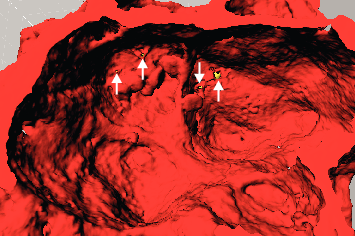
\includegraphics[height=\imsize]{img/XRM2008/imaris}\label{subfig:imaris}}\hfill
	\subfloat[]{\includegraphics[height=\imsize]{img/XRM2008/em/au900-1b-a}\label{subfig:slice-srxtm}}\hfill
	\subfloat[]{\includegraphics[height=\imsize]{img/XRM2008/em/au900-1b-b}\label{subfig:slice-em}}
	\caption[Three dimensional isosurface visualization of gold particles in the lung obtained from SRXTM data]{\subref{subfig:imaris}: Three dimensional isosurface visualization of gold particles in the lung obtained from \ac{SRXTM} data. Gold grains (yellow) are deposited in terminal airspaces. The air-tissue interface was removed on top of the gold grains during the visualization process in order to show the gold particles (arrows). \subref{subfig:slice-srxtm}: Detailed view of virtual \ac{SRXTM} section obtained at \ac{TOMCAT} containing two gold particles (arrows). The arrowheads are pointing to erythrocytes which are lighting up in the \ac{SRXTM} images due to their high iron content of the hemoglobin. Due to the high contrast of gold the particles appear larger in the \ac{SRXTM} images than they are in reality and we observed spiked image artifacts going out from the particles. \subref{subfig:slice-em}: Corresponding \ac{TEM} section of the virtual \ac{SRXTM} section. The thin black lines in \subref{subfig:slice-em} represent folds in the serial section. The white lines in \subref{subfig:slice-em} represent knife marks from the sectioning process.}
	\label{fig:imaris}
\end{figure}

\renewcommand{\imsize}{0.250\textwidth}
\begin{figure}[htb]
\centering
\subfloat[]{\includegraphics[width=\imsize]{img/XRM2008/em/au900-1b-c}\label{subfig:em-c}}\hfill
\subfloat[]{\includegraphics[width=\imsize]{img/XRM2008/em/au900-1b-d}\label{subfig:em-d}}\hfill
\subfloat[]{\includegraphics[width=\imsize]{img/XRM2008/em/au900-1b-e}\label{subfig:em-e}}\hfill
\subfloat[]{\includegraphics[width=\imsize]{img/XRM2008/em/au900-1b-f}\label{subfig:em-f}}\hfill
\caption[Transmission electron microscopy images of gold particles]{Transmission electron microscopy images of \SI{700}{\nano\meter} gold particles: \subref{subfig:em-c}--\subref{subfig:em-e}: Close-up view of square A of Fig.~\ref{subfig:slice-srxtm} showing a gold particle (arrows) in consecutive \ac{TEM} sections which are \SI{80}{\nano\meter} apart. \subref{subfig:em-f}: Gold grain observed in square B in Fig.~\ref{subfig:slice-srxtm} (arrow). Roughly half of the gold grains observed were located inside the cells, \eg macrophages. The thin black lines visible in subfigures \subref{subfig:em-c}, \subref{subfig:em-e} and \subref{subfig:em-f} represent folds in the \ac{TEM} section.}
\label{fig:srxtm-em}
\end{figure}

\section{Discussion}
A very high correlation between the two imaging modalities was observed. The virtual slices obtained from the \ac{SRXTM} image stack (Fig.~\ref{subfig:slice-srxtm}) and the real slices obtained using \ac{TEM} (Fig.~\ref{subfig:slice-em}) have only been corrected for rotation and magnification. The correct vertical position of the serial \ac{TEM} section in the sample was obtained through rigorous alignment and precise positioning of the sample in the microtome.

We have been able to track the gold particles over consecutive serial sections, even if they sometimes were not directly visible. As can be seen in Fig.~\ref{subfig:em-e}, we sometimes only observed a hole where we would have expected to see the gold particle (arrow). Since the gold grains are much harder than Epon and do not stick well to the resin, it is expected that the grains will be pulled out of the Epon block as soon as half of the grain is cut.

\section{Conclusions}
We conclude that the combination of \ac{SRXTM} and \ac{TEM} allows the three dimensional localization of particles in the mammalian lung. In a synergistic way, we used \ac{SRXTM} to obtain the full unrestricted \threed access and \ac{TEM} to verify the localization of the particles in the \threed-space with very high resolution. 

We are planning to use this method for the detection and localization of inhaled particles and as a mean of providing data for airflow simulation in the mammalian lung.

\section{Acknowledgments}
We thank Christoph Hinterm\"uller and Federica Marone for expert help at \ac{TOMCAT} and Bettina De Breuyn as well as Christoph Lehmann for the preparation of the samples. This work has been supported by Swiss National Science Foundation grant 3100A0-109874 and by US National Heart, Lung, and Blood Institute grant HL-070542.
%\bibliographystyle{plainnat}
%\label{app:bibliography} 
%\bibliography{../Bibliography,../../references,../Tsuda2008references}